% ============================================================================
%  YIP-BOI OS OPERATOR'S MANUAL
%  A Williams Tube PDA Operating System for VRChat
%  Styled after vintage spiral-bound computer manuals (C64, Apple II, TRS-80)
% ============================================================================
\documentclass[10pt]{article}

% --- Page geometry: wide landscape-ish spiral-bound notebook ---
% Target ~8.5 x 5.5" (half-letter, landscape feel)
\usepackage[
  paperwidth=8.5in,
  paperheight=5.5in,
  left=1.2in,          % extra left margin for spiral binding
  right=0.7in,
  top=0.6in,
  bottom=0.6in,
  headheight=12pt,
  headsep=8pt,
  footskip=20pt,
]{geometry}

% --- Fonts ---
\usepackage[T1]{fontenc}
\usepackage{inconsolata}
\renewcommand{\familydefault}{\ttdefault}

% --- Packages ---
\usepackage{xcolor}
\usepackage{graphicx}
\graphicspath{{assets/}}
\usepackage{fancyhdr}
\usepackage{titlesec}
\usepackage{enumitem}
\usepackage{tcolorbox}
\usepackage{booktabs}
\usepackage{hyperref}
\usepackage{microtype}
\usepackage{needspace}
\usepackage{float}
\usepackage{adjustbox}
\usepackage{parskip}
\usepackage{tikz}
\usepackage{etoolbox}

% --- Color Palette ---
\definecolor{crtgreen}{RGB}{51, 255, 51}
\definecolor{darkgreen}{RGB}{0, 100, 0}
\definecolor{screenbg}{RGB}{10, 20, 10}
\definecolor{mantitle}{RGB}{0, 80, 0}
\definecolor{rulecolor}{RGB}{0, 60, 0}
\definecolor{notebg}{RGB}{235, 245, 235}
\definecolor{warnbg}{RGB}{255, 245, 230}
\definecolor{warnborder}{RGB}{200, 120, 0}
\definecolor{spiralgray}{RGB}{140, 140, 140}
\definecolor{holebg}{RGB}{230, 230, 230}
\definecolor{pagebg}{RGB}{252, 250, 245}   % slightly warm off-white

% --- Page background color ---
\usepackage{eso-pic}
\AddToShipoutPictureBG{%
  \AtPageLowerLeft{%
    \color{pagebg}\rule{\paperwidth}{\paperheight}%
  }%
}

% --- Hyperlinks ---
\hypersetup{
  colorlinks=true,
  linkcolor=darkgreen,
  urlcolor=darkgreen,
}

% ============================================================================
% FIGURE HELPER
% ============================================================================
% \manualfig[width]{filename}{caption}
% If the image file doesn't exist, a placeholder box is drawn instead.
\newcommand{\manualfig}[3][0.8\textwidth]{%
  \begin{figure}[H]
    \centering
    \IfFileExists{assets/#2}{%
      \includegraphics[width=#1]{#2}%
    }{%
      \fcolorbox{spiralgray}{holebg}{%
        \parbox[c][1.5in]{#1}{%
          \centering\ttfamily\small\color{spiralgray}%
          [placeholder]\\[0.3em]%
          \footnotesize #2%
        }%
      }%
    }%
    \par\vspace{0.3em}
    {\footnotesize\ttfamily #3}
  \end{figure}
}

% ============================================================================
% SPIRAL BINDING DECORATION
% ============================================================================
\newcounter{spiralpage}
\newcommand{\drawspiral}{%
  \stepcounter{spiralpage}%
  \ifodd\value{spiralpage}%
    % Odd pages: spiral on the LEFT (like a right-hand page)
    \begin{tikzpicture}[remember picture, overlay]
      \foreach \i in {1,2,...,14} {
        \pgfmathsetmacro{\ypos}{\paperheight - \i * \paperheight / 15}
        \fill[holebg] ([xshift=0.42in, yshift=\ypos pt] current page.south west)
          circle (4pt);
        \draw[spiralgray, thick] ([xshift=0.42in, yshift=\ypos pt] current page.south west)
          circle (4pt);
        \draw[spiralgray, line width=1.2pt]
          ([xshift=0.42in, yshift=\ypos pt + 4pt] current page.south west)
          arc (90:270:4pt and 3pt);
      }
    \end{tikzpicture}%
  \else%
    % Even pages: spiral on the RIGHT (like a left-hand page)
    \begin{tikzpicture}[remember picture, overlay]
      \foreach \i in {1,2,...,14} {
        \pgfmathsetmacro{\ypos}{\paperheight - \i * \paperheight / 15}
        \fill[holebg] ([xshift=-0.42in, yshift=\ypos pt] current page.south east)
          circle (4pt);
        \draw[spiralgray, thick] ([xshift=-0.42in, yshift=\ypos pt] current page.south east)
          circle (4pt);
        \draw[spiralgray, line width=1.2pt]
          ([xshift=-0.42in, yshift=\ypos pt + 4pt] current page.south east)
          arc (90:-90:4pt and 3pt);
      }
    \end{tikzpicture}%
  \fi%
}

\AddToShipoutPictureFG{\drawspiral}

% ============================================================================
% HEADERS AND FOOTERS
% ============================================================================
\pagestyle{fancy}
\fancyhf{}
\fancyhead[L]{\small\texttt{YIP-BOI}}
\fancyhead[R]{\small\texttt{OPERATOR'S MANUAL}}
\fancyfoot[R]{\small\texttt{\thepage}}
\renewcommand{\headrulewidth}{0.5pt}
\renewcommand{\footrulewidth}{0pt}

% ============================================================================
% SECTION STYLING
% ============================================================================
\titleformat{\section}
  {\Large\bfseries\ttfamily\color{mantitle}}
  {\thesection.}{0.5em}{}
  [\vspace{-0.5em}\textcolor{rulecolor}{\rule{\textwidth}{1.2pt}}]

\titleformat{\subsection}
  {\large\bfseries\ttfamily}
  {\thesubsection}{0.5em}{}

\titleformat{\subsubsection}
  {\normalsize\bfseries\ttfamily}
  {\thesubsubsection}{0.5em}{}

\titlespacing*{\section}{0pt}{1.5em}{0.8em}
\titlespacing*{\subsection}{0pt}{1em}{0.4em}
\titlespacing*{\subsubsection}{0pt}{0.8em}{0.3em}

% ============================================================================
% CUSTOM ENVIRONMENTS
% ============================================================================

\newtcolorbox{screenbox}[1][]{
  colback=screenbg,
  colframe=darkgreen,
  coltitle=crtgreen,
  coltext=crtgreen,
  fontupper=\ttfamily\footnotesize,
  boxrule=1.5pt,
  arc=0pt,
  left=5pt, right=5pt, top=3pt, bottom=3pt,
  #1
}

\newtcolorbox{notebox}[1][NOTE]{
  colback=notebg,
  colframe=darkgreen,
  fonttitle=\bfseries\ttfamily\small,
  title={#1},
  boxrule=0.8pt,
  arc=0pt,
  left=5pt, right=5pt, top=2pt, bottom=2pt,
}

\newtcolorbox{warnbox}[1][IMPORTANT]{
  colback=warnbg,
  colframe=warnborder,
  fonttitle=\bfseries\ttfamily\small,
  title={#1},
  boxrule=0.8pt,
  arc=0pt,
  left=5pt, right=5pt, top=2pt, bottom=2pt,
}

\newcommand{\key}[1]{\fbox{\texttt{\footnotesize #1}}}

% ============================================================================
\begin{document}

% ============================================================================
% INSIDE FRONT COVER (copyright page)
% ============================================================================
\thispagestyle{empty}
\vspace*{\fill}
\begin{center}
{\footnotesize\ttfamily
Copyright \copyright\ 2026 by Foxipso Business Machines, Inc.\\
All rights reserved.\\[1em]
This manual is copyrighted and contains proprietary information. This publication
can generally be reproduced, stored in a retrieval system, or transmitted in any
form or by any means, electronic, mechanical, photocopying, recording or otherwise,
without the prior written permission of FOXIPSO BUSINESS MACHINES, Inc., provided
it remains unmodified.\\[1em]
First Edition --- March 2026\\
Part No. FBM-YB-001-EN
}

\vspace{1em}
\IfFileExists{assets/FBM logo.png}{%
  \includegraphics[width=0.25\textwidth]{FBM logo.png}%
}{}
\end{center}
\vspace*{\fill}

% ============================================================================
% TITLE PAGE
% ============================================================================
\newpage
\thispagestyle{empty}
\vspace*{0.3in}
\begin{center}

{\Huge\bfseries\ttfamily\color{mantitle}
YIP-BOI}

\vspace{0.3em}
{\Large\bfseries\ttfamily\color{mantitle}
OPERATOR'S MANUAL}

\vspace{0.6em}
\textcolor{rulecolor}{\rule{0.7\textwidth}{1.5pt}}

\vspace{0.4em}
{\normalsize\ttfamily
YIP-BOI Personal Data Assistant\\
Wrist-Mounted CRT Terminal --- Model YB-1}

\vspace{0.5em}

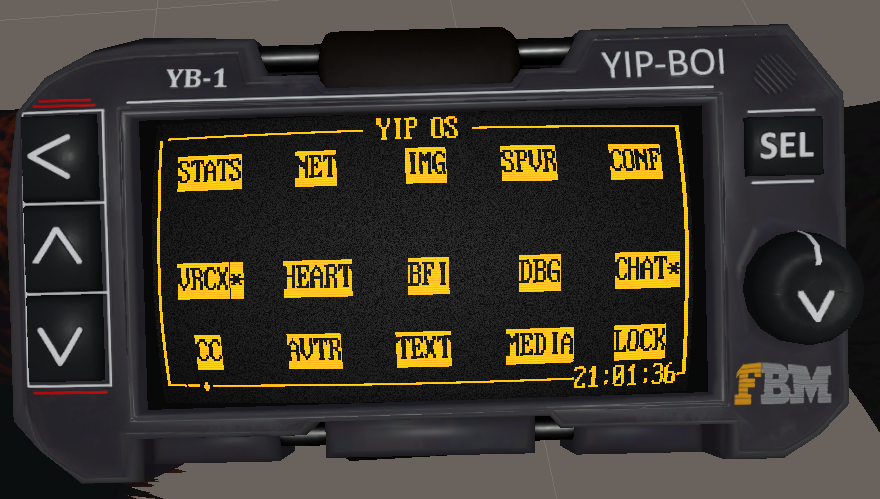
\includegraphics[width=0.55\textwidth]{YIP-BOI.png}

\vspace{0.5em}
{\small\ttfamily
For use with the Yip OS Desktop Companion Application\\[0.3em]
Revision 1.0.3}

\vspace{0.4em}

{\footnotesize\ttfamily
FOXIPSO BUSINESS MACHINES}

\end{center}
\vfill

% ============================================================================
% TABLE OF CONTENTS
% ============================================================================
\newpage
\thispagestyle{fancy}

\begin{center}
{\Large\bfseries\ttfamily\color{mantitle} TABLE OF CONTENTS}
\end{center}
\vspace{0.5em}

\renewcommand{\contentsname}{}
\setcounter{tocdepth}{2}
{\small
\makeatletter
\@starttoc{toc}
\makeatother
}

% ============================================================================
% BLANK PAGE
% ============================================================================
\newpage
\thispagestyle{fancy}
\vspace*{\fill}
\begin{center}
{\small\ttfamily THIS PAGE UNINTENTIONALLY LEFT BLANK}
\end{center}
\vspace*{\fill}

% ============================================================================
% INTRODUCTION
% ============================================================================
\newpage
\section{INTRODUCTION}
\label{sec:intro}

\subsection{Welcome}

Thank you for purchasing a Foxipso Yip-Boi from your authorized Foxipso Business Machines dealer. As you unpack and set up your device you should read through this instruction manual to get familiar with your brand new piece of personal computing technology.

\subsection{Features}

Your Yip-Boi features a \textbf{CRT screen} (green, amber, white, blue --- you can customize it like crazy), which renders data in beautiful monochrome, has a \textbf{touchscreen interface}, packs an \textbf{expandable 4K graphical ROM}, \textbf{256-character font set}, and even beeps with a \textbf{PC speaker}! It straps to your arm using a blendshape-equipped, possibly sustainably sourced leather band\footnote{We've made every reasonable attempt to remove any tattoos, matcaps, glitter effects, or e-boy scent from the leather band, but we do not guarantee such a condition.} that won't pinch and tug at your fur.

\subsection{Interaction}

Your Yip-Boi is designed to be worn around your \textbf{left arm}, and allows you --- and your friends! --- to view and interact with an \textbf{unlimited quantity} (not predetermined at upload time) of real data and bona fide programs. It features a touchscreen display with a realistic CRT shader and \textbf{six touch points}, housed in an arguably radiation-resistant enclosure that has \textbf{five physical buttons}. Interaction is accomplished by tapping the tippy tip of your right or left index finger claw-tip against these various contact points. E-boy/e-girl nail-tips may possibly work, but are untested. A very vertical inclination of your paw and index finger is highly recommended, to avoid accidental presses.

\subsection{How It Works}

Your new Yip-Boi is designed to work with \textbf{Yip OS}, a free and open-source operating system that runs on your computer as an OSC app. Your arm-worn Yip-Boi is mostly a display computer, and at its heart --- although invisible to players --- is a contraption called a \textbf{Williams Tube}: it's a VRChat camera and glyph-based write head that's inspired by the real historical device, which was one of the earliest examples of RAM storage and retrieval.

When you're in a VRChat world, the Yip OS desktop app is continually sending OSC control commands to this invisible camera and write head that are floating near your avatar; the commands are designed in such a way to rapidly render font glyphs and graphics from a ROM that's stored as textures contained in a custom shader in the Williams Tube asset.

Via the combination of these two prefabs, you can easily have a real computer on your wrist, fully interactive while in VRChat, that's capable of arbitrary computing tasks!

\input{williams_tube_diagram}

\input{yipboi_contacts_diagram}

% ============================================================================
% SETUP
% ============================================================================
\newpage
\section{SETUP}
\label{sec:setup}

\subsection{Unity Installation}

Unzip your Yip-Boi \texttt{.zip} file and drag the \texttt{.unitypackage} into your Unity project. FBM recommends creating a backup with ALCOM or VCC.

\begin{warnbox}[NOTE]
The Williams Tube rendering method requires \textbf{27 bits of parameter space}. This is fairly heavy for an asset, and you may want to make a version of your avatar that sacrifices some of your other heavy assets.
\end{warnbox}

\begin{enumerate}[leftmargin=2em]
  \item Open \texttt{Foxipso/Assets/Yip-Boi} in the Project View and drag the \texttt{Yip-Boi} prefab onto your avatar.
  \item Locate \texttt{Yip-Boi->Container} in the Hierarchy View and position and scale it as desired.
\end{enumerate}

You can now upload your avatar and test in VRChat. See Section~\ref{sec:companion} for the companion software.

\subsection{Testing in Unity}
\label{sec:testing}

It's possible to test the asset in Unity using lyuma's Av3Emulator and OSC mode, or the included OSC scripts. This is convenient for tweaking the look of the CRT or familiarizing yourself with the operation of the device prior to being in VR.

Testing with the included OSC scripts is easiest, and the use of Av3Emulator is a bit out of scope. To test:

\begin{enumerate}[leftmargin=2em]
  \item Recommended: Disable VRCFury in Play Mode by going to \texttt{Tools->VRCFury->Settings->Enable VRCFury in Play Mode}. This makes testing faster and means you don't have to navigate menus in Gesture Manager or Av3Emulator.
  \item Locate \texttt{Yip-Boi->Williams Tube->Play Mode Debugger (Removes On Upload)} in the Hierarchy View. In the Inspector, change the Tag from ``EditorOnly'' to ``Untagged''. This allows the OSC scripts to run in Play mode.
  \item Enter Play mode and look at the Yip-Boi. Start Yip OS.
  \item When finished testing, go back to \texttt{Yip-Boi->Williams Tube->Play Mode Debugger (Removes On Upload)} in the Hierarchy View and change the Tag back to ``EditorOnly''. If you forget, the two OSC testing scripts will prevent your avatar from uploading.
\end{enumerate}

You should now see the boot screen followed by the Home screen. After a timeout, you'll see the lock icon appear in the status bar on the bottom-left of the Yip OS screen. You can disable lock mode by pressing \key{SEL} three times. See Section~\ref{sec:conf} to learn about the CONF program and ALOCK.

\subsubsection{Virtual Buttons}

You can interact with Yip OS using virtual buttons in the \textbf{Status} tab of the Yip OS desktop application. Click the on-screen buttons to simulate VRChat interaction, or use the following keyboard shortcuts:

\begin{center}
{\small
\begin{tabular}{lll}
  \toprule
  \textbf{Keys} & \textbf{Row} & \textbf{Touch Zones} \\
  \midrule
  \key{1}--\key{5} & Row 1 & Top row (5 zones) \\
  \key{Q}--\key{T} & Row 2 & Middle row (5 zones) \\
  \key{A}--\key{G} & Row 3 & Bottom row (5 zones) \\
  \key{F1}--\key{F5} & --- & Physical buttons \\
  \bottomrule
\end{tabular}
}
\end{center}

\subsubsection{Exploring Programs}

Try various programs and familiarize yourself with navigation. See Section~\ref{sec:display} for the user interface, Section~\ref{sec:programs} for program operation, and Section~\ref{sec:nvram} for NVRAM. Any changes you make here will persist and be available in-game.

Now would be a good time to configure:
\begin{itemize}[leftmargin=2em, nosep]
  \item Your \textbf{VRCX} SQLite database path (see Section~\ref{sec:vrcx})
  \item The \textbf{CC} closed captions program (see Section~\ref{sec:cc})
  \item \textbf{AVTR} avatar management (see Section~\ref{sec:avtr})
\end{itemize}

\subsubsection{Customizing the CRT}

If you wish to customize the look of the CRT, click on \texttt{Yip-Boi->Container->Wrist CRT} in the Hierarchy View and scroll down to the \texttt{YB-1 (Material)} section. Click to unlock the shader, if necessary. Scroll down to \texttt{Special FX->CRT Screen} and experiment with changes there.

Recommended parameters to try: Font Color, Background Color, Static Noise, Jitter, Phosphor Persistence, Flickering, Horizontal Sync, and Bloom Glow.

\manualfig[0.4\textwidth]{SHADER OPTIONS.png}{CRT Screen shader options in the YB-1 material Inspector.}

\subsection{Connecting to VRChat}

The Yip-Boi communicates with VRChat using \textbf{OSC Query}, a service discovery protocol that lets VRChat and Yip OS find each other automatically. No manual port configuration is needed.

\textbf{Setup procedure:}

\begin{enumerate}[leftmargin=2em]
  \item Enable OSC in VRChat: Action Menu $\rightarrow$ Options $\rightarrow$ OSC $\rightarrow$ Enabled
  \item Upload your avatar with the Yip-Boi prefab installed
  \item Launch the Desktop Companion application on your PC
  \item VRChat will discover Yip OS via mDNS and establish a bidirectional connection
  \item The PDA display will begin rendering within a few seconds
  \item Confirm connection by checking for the spinning cursor (see Section~\ref{sec:spinner})
\end{enumerate}

\begin{notebox}
OSC Query is enabled by default. To disable it, set \texttt{query\_enabled = false} under the \texttt{[osc]} section in \texttt{config.ini}. When disabled, the companion app falls back to static UDP ports (send to 9000, listen on 9001) and you must ensure OSC routing is configured correctly yourself.
\end{notebox}

\subsubsection{Manual OSC Routing (Fallback)}

If OSC Query is unavailable or disabled, Yip OS uses static ports:

\begin{center}
{\small
\begin{tabular}{lll}
  \toprule
  \textbf{Port} & \textbf{Direction} & \textbf{Purpose} \\
  \midrule
  9000 & Companion $\rightarrow$ VRChat & Display writes \\
  9001 & VRChat $\rightarrow$ Companion & Input events \\
  \bottomrule
\end{tabular}
}
\end{center}

If you have multiple OSC programs running, you may need an OSC router such as VOR or VRCOSC. Create a new entry in your router, assign a new port (e.g., 9010), and set this port in the \textbf{``OSC'' tab} of the desktop app under \textbf{``Listen Port.''} It's generally not necessary to change Send Port.

\manualfig[0.55\textwidth]{osc tab.png}{The OSC configuration tab in the Yip OS desktop app. These settings are only needed when OSC Query is disabled.}

\subsection{The Boot Sequence}

When the companion software starts, the Yip-Boi performs a boot sequence. A progress bar fills across the screen as the system initializes. The speed of the boot animation is configurable (see Section~\ref{sec:conf}).

Upon completion, the Home screen will appear. You are now ready to operate your Yip-Boi.

% ============================================================================
% PHYSICAL CONTROLS
% ============================================================================
\newpage
\section{PHYSICAL CONTROLS}
\label{sec:controls}

\manualfig[0.7\textwidth]{Yip-Boi overview.png}{Physical layout of the Yip-Boi PDA, Model YB-1.}

The Yip-Boi PDA has two types of input: \textbf{physical buttons} on the device housing, and \textbf{touchscreen contacts} on the display surface.

\begin{notebox}
All input currently requires either your left or right index fingers. A possible future improvement is to require a specific gesture on either or both paws, if users end up causing too many errant inputs. In the meantime, the \textbf{LOCK} program (see Section~\ref{sec:lock}) and the \textbf{AUTOLOCK} feature in CONF (see Section~\ref{sec:conf}) are recommended to prevent accidental inputs.
\end{notebox}

\begin{warnbox}
\textbf{ALOCK (Autolock) is enabled by default.} If you find that your inputs aren't registering, check the bottom-left of the status bar for the lock icon. If visible, press \key{SEL} three times rapidly to unlock. You can adjust or disable autolock timing in the CONF program (see Section~\ref{sec:conf}).
\end{warnbox}

\subsubsection{Disabling the Beep}

The Yip-Boi produces an audible beep on input via an Audio Source component. To disable or customize this:

\begin{enumerate}[leftmargin=2em, nosep]
  \item Locate \texttt{1. Yip-Boi->Container->Wrist CRT} in the Hierarchy.
  \item Locate \texttt{Audio Source} in the Inspector and click the \texttt{Mute} checkbox.
  \item You can also replace the sound effect with your own choice here.
\end{enumerate}

\begin{notebox}
This isn't a configurable option in-game because that would use another bit of synced parameter space.
\end{notebox}

\subsection{Buttons}

Five physical controls are mounted on the device. Their names in this manual correspond to the labels shown in the overview diagram above.

\begin{description}[style=nextline, leftmargin=1em, font=\bfseries\ttfamily]
  \item[BACK (Top Left)]
    Your primary navigation control. Press to go back one screen, up to the HOME screen. A \textbf{left arrow} ($\leftarrow$) on the top of the left border indicates when BACK is available.

  \item[PAGE UP (Middle Left)]
    Scrolls or pages up on screens with multiple pages. An \textbf{up arrow} ($\uparrow$) on the middle of the left border indicates when this is available.

  \item[PAGE DOWN (Bottom Left)]
    Scrolls or pages down. A \textbf{down arrow} ($\downarrow$) on the bottom of the left border indicates availability.

  \item[SEL (Top Right)]
    Select. Performs a context-sensitive action depending on the current screen. Often used to select the currently highlighted item in a list. A \textbf{right arrow} ($\rightarrow$) on the top of the right border indicates when SEL can be used.

  \item[SCROLL DOWN / Joystick (Bottom Right)]
    Cycles downward through list items, wrapping around to the top. A simple push-to-toggle button --- no directional input.
\end{description}

\subsection{Touchscreen}

The display surface is divided into a \textbf{5$\times$3 grid} of touch zones (15 total). Which zones are active depends on the current screen.

\manualfig[0.55\textwidth]{touch points.png}{Touchscreen contact point locations on the display surface.}

All inputs are debounced with a configurable window. This prevents double-taps, which matters when your index finger is fighting with VR tracking for positional accuracy. It's generally recommended to use \textbf{LONG} or \textbf{NORM} debouncing. You can edit this in the CONF program (see Section~\ref{sec:conf}).

% ============================================================================
% UNDERSTANDING THE DISPLAY
% ============================================================================
\newpage
\section{UNDERSTANDING THE DISPLAY}
\label{sec:display}

Yip OS programs use consistent visual conventions across every screen.

\manualfig[0.7\textwidth]{Screen overview.png}{Screen element overview (STATS program shown).}

\subsection{Screen Layout}

Programs generally lay out their content in the same structure. The display is a 40-column by 8-row character grid. Columns 0 and 39 are reserved for the border. Row 0 is the title bar. Row 7 is the status bar. That leaves rows 1--6 (228 cells) for content.

\subsection{The Borders}

The outside border of the screen displays useful navigation information:

\textbf{Left border:}
\begin{description}[style=nextline, leftmargin=1em, font=\bfseries\ttfamily, nosep]
  \item[Top] A left arrow indicating when BACK can be used.
  \item[Middle] An up arrow indicating when PAGE UP can be used.
  \item[Bottom] A down arrow indicating when PAGE DOWN can be used.
\end{description}

\textbf{Right border:}
\begin{description}[style=nextline, leftmargin=1em, font=\bfseries\ttfamily, nosep]
  \item[Top] A right arrow indicating the SEL button can be used, often to select an item in a list.
\end{description}

\manualfig[0.7\textwidth]{Screen Overview 2.png}{Border indicators, page counter, and list selection (AVTR CHANGE screen shown).}

\subsection{The Status Bar}

The bottom border (row 7) contains, from left to right:

\begin{description}[style=nextline, leftmargin=1em, font=\bfseries\ttfamily, nosep]
  \item[Spinnyboi (col 1)]
    \label{sec:spinner}
    The friendly \texttt{| / - \textbackslash} animation. Acts as a heartbeat and constant companion, indicating that Yip OS is alive and updating the display. If it stops spinning, the connection may have been interrupted.

  \item[Lock indicator (col 2)]
    When visible, indicates the autolock is active. When \textbf{inverted}, it shows that input was attempted but prevented by lock mode. Press \key{SEL} three times rapidly to unlock. See Section~\ref{sec:lock}.

  \item[Notification dot (col 3)]
    A bullet ($\bullet$) indicates a program has a notification to display. Go BACK to the Home screen and tap the program name that has an \texttt{*} next to it to navigate to the notification. Currently VRCX and CHAT generate notifications.

  \item[Page indicator]
    On multi-page screens, displays the current page and total (e.g., ``1/5'').

  \item[System clock (right side)]
    Your computer's local time, in 24-hour \texttt{HH:MM:SS} format. Normally visible, except on visually intense screens that require the highest refresh rates (e.g., the CC display --- see Section~\ref{sec:cc}).
\end{description}

\subsection{Inverted Text = Touchable}
\label{sec:inverted}

\begin{warnbox}
This is the most important rule in Yip OS: \textbf{if text appears in inverted video (light background, dark characters), you can touch it.} Inverted text always means ``this is a button.''
\end{warnbox}

Programs will display touchscreen buttons in inverted (highlighted) text. Carefully tap the very tip of your claw against the button to select it. The button will flash in un-inverted text before performing an operation. For example, the DSK button in STATS will cycle through which mountpoint/disk is displayed in the graph. (Your selection will persist in NVRAM. See Section~\ref{sec:nvram}.)

\subsection{List Selection}

Programs may also provide you with a list of items from which to make a selection. In these cases, the currently selected item will be indicated by the first three characters being inverted. Press \key{JOYSTICK} to cycle down through the items, or to wrap around to the top. Press \key{SEL} to select an item.

\subsection{NVRAM}
\label{sec:nvram}

In some cases, selections you make will persist to memory. Yip OS provides \textbf{NVRAM} that stores information between power cycles. To clear this memory and revert any configuration changes or selections you've made, go to CONF page 1, tap NVRAM, then tap again to confirm.

% ============================================================================
% HOME SCREEN
% ============================================================================
\newpage
\section{HOME SCREEN}
\label{sec:home}

Yip OS boots into the Home screen after displaying a brief boot graphic. The Home screen displays a grid of program tiles corresponding to the touchscreen zones. Tap a tile to launch that program.

\manualfig[0.55\textwidth]{HOME.png}{The Home screen with active program tiles. (Programs seen here that aren't highlighted weren't available in that version of Yip OS.)}

\subsection{Tile Grid}

\textbf{Page 1:}
\begin{center}
{\small
\begin{tabular}{c|ccccc}
  \toprule
  & \textbf{Col 1} & \textbf{Col 2} & \textbf{Col 3} & \textbf{Col 4} & \textbf{Col 5} \\
  \midrule
  \textbf{Row 1} & STATS & NET & IMG & SPVR & CONF \\[0.3em]
  \textbf{Row 2} & VRCX & HEART & BFI & STONK & CHAT \\
  \textbf{Row 3} & CC & AVTR & TEXT & MEDIA & LOCK \\
  \bottomrule
\end{tabular}
}
\end{center}

\textbf{Page 2:}
\begin{center}
{\small
\begin{tabular}{c|ccccc}
  \toprule
  & \textbf{Col 1} & \textbf{Col 2} & \textbf{Col 3} & \textbf{Col 4} & \textbf{Col 5} \\
  \midrule
  \textbf{Row 1} & DBG & ----- & ----- & ----- & ----- \\[0.3em]
  \textbf{Row 2} & ----- & ----- & ----- & ----- & ----- \\
  \textbf{Row 3} & ----- & ----- & ----- & ----- & ----- \\
  \bottomrule
\end{tabular}
}
\end{center}

Active tiles are displayed in \textbf{inverted text} (touchable). Tiles marked ``-----'' are reserved for future programs and do not respond to input. Use \textbf{PG UP / PG DWN} (ML / BL buttons) to switch between pages. A page indicator (e.g. ``1/2'') is shown in the status bar.

These programs have functions that can run in the background and are launchable from the Home screen.

\subsection{Navigation}

Tapping an active tile:
\begin{enumerate}[leftmargin=2em, nosep]
  \item The tile flashes (un-inverts) confirming your touch
  \item After $\sim$300ms, the program screen loads
  \item Display clears, stamps the macro background, renders dynamic content
\end{enumerate}

From any program, press \key{BACK} to return to the previous screen. Press it repeatedly to return to Home.

% ============================================================================
% PROGRAMS
% ============================================================================
\newpage
\section{PROGRAMS}
\label{sec:programs}

By default, Yip OS v1.0 comes with the following programs:

\subsection{STATS --- System Monitor}
\label{sec:stats}

Displays your CPU and GPU utilization, system and GPU temperatures, memory usage, network throughput, disk usage, system uptime, and Yip OS uptime.

\manualfig[0.55\textwidth]{STATS.png}{The STATS program displaying system metrics.}

The Stats program refreshes automatically. No touch interaction required --- just glance at your wrist. The \textbf{DSK} button (inverted, touchable) cycles through which mountpoint/disk is displayed in the disk usage graph.

\newpage
\subsection{NET --- Network Monitor}
\label{sec:net}

Displays a real-time bar graph of your system's network utilization using an oscilloscope-style sweep rendering.

\manualfig[0.55\textwidth]{NET graph example.png}{The NET program with oscilloscope sweep graph.}

The graph uses a circular buffer with a sweep cursor. New data writes at the cursor position, and a two-column clear gap moves ahead of it, creating the classic oscilloscope sweep effect.

\textbf{The interface name} (e.g., ``eth0'') is displayed in inverted text. Tap it to cycle through available network interfaces.

\subsubsection{Graph Scale Indicator}

The Y-axis range is shown by a scale indicator at the bottom-left of the graph area. The bottom of the graph always represents 0~B/s. The top initially represents 2~kB/s.

The scale indicator starts at ``\texttt{0}'' and increments through \texttt{0--9, A--Z} each time the graph auto-scales. A \textbf{scale-change marker} is drawn at the column where the new scale takes effect, letting you see when and where throughput spikes caused rescaling.

\newpage
\subsection{HEART --- Heartbeat Monitor}
\label{sec:heart}

A real-time heartbeat monitor and graph via OSC. Uses the same oscilloscope sweep rendering as the NET program. Displays current BPM, session high, low, and average.

\manualfig[0.55\textwidth]{HEART.png}{The HEART program displaying heartbeat data.}

\begin{notebox}
The Yip-Boi receives BPM data from an OSC-based heart rate monitor or other external source. You can test the display using the \textbf{Simulate OSC Input} feature in the desktop app's OSC tab, which sends a configurable heart rate value at 1~Hz.
\end{notebox}

\newpage
\subsection{SPVR --- StayPutVR}
\label{sec:stay}

Integration with Foxipso's StayPutVR, allowing you or friends to lock/unlock your VR-tracked devices and control shockers or other devices.

\manualfig[0.55\textwidth]{SPVR.png}{The SPVR program with body part toggles.}

Each body part label is displayed in inverted text (touchable). Tap a label to toggle its lock state.

\newpage
\subsection{CONF --- Configuration}
\label{sec:conf}

A config utility for modifying various settings that control the operation and behavior of the device and OS. Spans multiple pages --- use \key{PAGE UP} and \key{PAGE DOWN} to navigate.

\manualfig[0.55\textwidth]{CONFIG1_2.png}{CONF program, page 1 of 2.}

\manualfig[0.55\textwidth]{CONFIG2_2.png}{CONF program, page 2 of 2.}

Setting labels are inverted (touchable). Tap to cycle through values. Settings persist to \texttt{config.ini} and survive restarts.

\begin{center}
{\small
\begin{tabular}{lll}
  \toprule
  \textbf{Parameter} & \textbf{Values} & \textbf{Description} \\
  \midrule
  BOOT & OFF / SLOW / NORM / FAST & Boot animation speed \\
  WRITE & ULTR / FAST / NORM / SLOW & Character write delay \\
  SETTLE & NORM / SLOW / FAST & Mode switch settle delay \\
  LOG & DBG / INFO / WARN / ERR & Log verbosity level \\
  DBNCE & NORM / LONG / SHRT & Touch debounce timing \\
  NVRAM & CLR / SUR? / CLR & Clear stored settings \\
  REFR & OFF / 5 / 10 / 30 & Auto-refresh interval (sec) \\
  ALOCK & OFF / 10S / 30S / 1M & Autolock timeout \\
  CHATBG & OFF / 30S / 1M / 5M & CHAT background poll rate \\
  REBOOT & GO! & Restart the system \\
  \bottomrule
\end{tabular}
}
\end{center}

\begin{notebox}
\textbf{REFR} defaults to \textbf{30S} and is recommended to be left on. It periodically clears and redraws the display, which corrects visual artifacts caused by VRChat UI elements clipping into the camera or other in-game interference. \textbf{ALOCK} is enabled by default to prevent accidental inputs. \textbf{CHATBG} sets how frequently the CHAT program checks for new messages in the background (see Section~\ref{sec:chat}).
\end{notebox}

\begin{notebox}
\textbf{WRITE} and \textbf{SETTLE} are important parameters that affect display quality and remote visibility. See Section~\ref{sec:performance} for details on write speed and reliability.
\end{notebox}

\newpage
\subsection{VRCX}
\label{sec:vrcx}

Read-only integration into VRCX's SQLite database, allowing you to see notifications, a feed of your friends going online/offline, and your recent world history. You can also launch a browser to rejoin recent instances.

\manualfig[0.55\textwidth]{VRCX.png}{VRCX hub screen --- tap a category to view its contents.}

The VRCX hub provides access to three sub-screens:

\textbf{Feed} --- Shows a real-time activity feed of your friends going online and offline, with timestamps.

\manualfig[0.55\textwidth]{VRCX_FEED.png}{VRCX friend activity feed. Use \key{JOYSTICK} to scroll, \key{SEL} to view friend details.}

\textbf{Worlds} --- Lists your recent world history. Select a world to view details and optionally launch a browser to rejoin the instance.

\manualfig[0.55\textwidth]{VRCX_WORLDS.png}{VRCX recent worlds list.}

\begin{notebox}
Yip OS can only display standard ASCII characters. Friend names or world names containing special or Unicode characters will appear garbled on the display.
\end{notebox}

\textbf{Notifications} --- Displays your pending VRCX notifications (friend requests, invites, etc.).

\manualfig[0.55\textwidth]{VRCX_NOTIF.png}{VRCX notifications screen.}

When VRCX has unseen notifications, an \texttt{*} appears next to the VRCX tile on the Home screen, and a notification dot ($\bullet$) appears in the status bar.

\newpage
\subsection{CC --- Closed Captions}
\label{sec:cc}

A locally running closed captions program powered by Georgi Gerganov's \textbf{whisper.cpp} (\url{https://github.com/ggml-org/whisper.cpp/}). It listens to your system audio or your selected microphone and displays live transcription on the CRT. This is one of the most visually intensive programs --- the status bar clock may be temporarily hidden to maximize refresh rate.

\manualfig[0.55\textwidth]{CC.png}{CC program displaying live transcription. Text scrolls upward as new speech is detected.}

The CC display uses a \textbf{sliding window} approach for streaming transcription. Audio is processed in overlapping windows, producing progressive tentative text that refines before being finalized.

At \textbf{ULTRA write speed}, the display is split into two zones:
\begin{itemize}
  \item \textbf{Rows 1--4} (normal text): Finalized transcription. Text scrolls upward as new lines are committed.
  \item \textbf{Rows 5--6} (inverted text): Tentative transcription preview. This text updates in-place as the model refines its output, then clears when the text is finalized and moves to the committed zone above.
\end{itemize}

\noindent At \textbf{NORM} or \textbf{SLOW} write speeds, the tentative zone is disabled and all six rows are used for finalized text only, since the slower refresh rate cannot keep up with progressive updates.

The transcription model runs entirely on your local machine --- no audio is sent to external servers. Inference uses \textbf{Vulkan GPU acceleration} on NVIDIA and AMD GPUs, with automatic CPU fallback if no compatible GPU is available. On Linux, audio capture uses \textbf{PulseAudio}.

Due to the CRT's ASCII-only character set, all transcription output is \textbf{automatically translated to English}. Non-English speech is translated in real time; English speech passes through unchanged. This means CC functions as both a captioning and a live translation tool.

\subsubsection{Model Installation}

CC requires a GGML-format Whisper.cpp model. Download one from:

\begin{quote}
\url{https://huggingface.co/ggerganov/whisper.cpp/tree/main}
\end{quote}

\noindent Place the \texttt{.bin} file in the \texttt{models} directory:

\begin{center}
{\small
\begin{tabular}{ll}
  \toprule
  \textbf{Platform} & \textbf{Path} \\
  \midrule
  Windows & \texttt{\%APPDATA\%\textbackslash yip\_os\textbackslash models\textbackslash} \\
  Linux & \texttt{\~{}/.config/yip\_os/models/} \\
  \bottomrule
\end{tabular}
}
\end{center}

The model file must be named \texttt{ggml-\textit{<model>}.bin} (e.g., \texttt{ggml-tiny.en.bin}). All installed models appear in a dropdown in the \textbf{CC tab} of the desktop app. FBM recommends \textbf{base.en} for English-only use, or a multilingual model such as \textbf{large-v3-turbo} for translation. With Vulkan GPU acceleration, even larger models run comfortably in real time.

\manualfig[0.55\textwidth]{CC_CONF.png}{CC configuration screen --- select audio source and model size.}

The CC configuration screen allows you to select your \textbf{audio input source} (system audio or a specific microphone) and the \textbf{Whisper model size} (from the models you've downloaded).

\begin{notebox}
Log files are stored in the \texttt{logs} directory alongside \texttt{models}:
\texttt{\%APPDATA\%\textbackslash yip\_os\textbackslash logs\textbackslash} (Windows) or \texttt{\~{}/.config/yip\_os/logs/} (Linux). Check \texttt{yip\_os.log} if CC or any other feature isn't working as expected.
\end{notebox}

\newpage
\subsection{AVTR --- Avatar Manager}
\label{sec:avtr}

An OSC application that reads your VRChat cached avatars and OSC config and allows you to change avatars and enable/disable your toggles --- all from your wrist.

\manualfig[0.55\textwidth]{AVTR.png}{AVTR hub --- choose to change avatars or control toggles.}

The AVTR hub provides two functions:

\textbf{CHANGE} --- Browse and switch between your cached avatars. The list shows all avatars that VRChat has cached OSC data for, not just your favorites. Note that VRChat only allows switching to \textbf{favorited} avatars via OSC --- if the avatar is not in your favorites, the change will be silently ignored.

\manualfig[0.55\textwidth]{AVTR_CHANGE.png}{Avatar selection list. Use \key{JOYSTICK} to cycle, \key{SEL} to view details.}

\begin{notebox}
Yip OS can only display standard ASCII characters. Avatar names containing special or Unicode characters (e.g., Japanese, emoji, accented letters) will appear garbled on the display.
\end{notebox}

\manualfig[0.55\textwidth]{AVTR_DETAIL.png}{Avatar detail view --- press \key{SEL} to switch to this avatar.}

\textbf{CTRL} --- View and toggle parameters on your current avatar. The toggle list is populated from your avatar's radial menu parameters (via LocalAvatarData), so it shows all expression parameters --- not just simple on/off toggles. Parameters that are not Bool toggles may not respond as expected.

\manualfig[0.55\textwidth]{AVTR_CTRL.png}{Toggle controls for the current avatar. Tap inverted labels to toggle.}

\newpage
\subsection{LOCK --- Screen Lock}
\label{sec:lock}

Locks out all input until you tap \key{SEL} three times. Useful for preventing accidental input.

\manualfig[0.55\textwidth]{LOCK.png}{The LOCK screen.}

\manualfig[0.55\textwidth]{HOME_LOCKED.png}{Home screen with lock indicator active in the status bar.}

\manualfig[0.55\textwidth]{HOME_LOCK_FLASH.png}{Lock indicator flashing (inverted) when blocked input is attempted.}

When locked, the lock icon appears in the status bar (col 2). If someone attempts input while locked, the lock icon briefly \textbf{inverts} (flashes) to indicate the input was blocked.

\newpage
\subsection{BFI --- BrainFlow Monitor}
\label{sec:bfi}

Integration with \textbf{BFiVRC} by ChilloutCharles (\url{https://github.com/ChilloutCharles/BrainflowsIntoVRChat}), which connects the BrainFlow Library to EEG hardware and outputs brain--computer interface parameters via OSC.

\manualfig[0.55\textwidth]{BFIVRC.png}{The BFI program displaying a live parameter graph with oscilloscope sweep rendering.}

The BFI program displays a real-time graph of the selected BFiVRC parameter, using the same oscilloscope sweep rendering as NET and HEART. The current parameter name is shown at the bottom-left, and a \textbf{CONF} button (inverted, touchable) is available to access BFI-specific settings.

\manualfig[0.55\textwidth]{BFI PARAM.png}{BFI parameter selection --- use \key{JOYSTICK} to cycle, \key{SEL} to select.}

Press \key{SEL} from the graph view to open the parameter selection list. Use \key{JOYSTICK} to cycle through available BFiVRC parameters (e.g., FocusAvg, FocusPosAvg, FocusLeft, etc.) and \key{SEL} to select which parameter to graph.

\begin{notebox}
You do not need EEG hardware to preview the BFI display. The Yip OS desktop app provides a \textbf{Simulate OSC Input} feature (in the OSC tab) that sends synthetic sine wave data for all 26 BFiVRC parameters, as well as simulated heart rate data.
\end{notebox}

\manualfig[0.55\textwidth]{Simulate OSC input for heartrate and BFI.png}{The Simulate OSC Input panel in the desktop app --- generates test data for BFI and heart rate.}

\newpage
\subsection{CHAT --- Telegram Group Chat}
\label{sec:chat}

A live group chat viewer for \textbf{@YipBoiChat} on Telegram. People who purchased the Yip-Boi asset get access to this Telegram group, and anyone with the device can view messages live in VRChat directly on their wrist.

\manualfig[0.55\textwidth]{CHAT.png}{The CHAT program displaying recent messages with sender names and timestamps.}

\manualfig[0.55\textwidth]{CHAT CONSENT.png}{CHAT consent screen --- tap I CONSENT to accept and begin viewing messages.}

On first launch, CHAT displays a consent screen. Once accepted, the program fetches messages from a Cloudflare Worker endpoint using a simple HTTP request --- no Telegram account, API key, or credentials are required to read the public chat room.

Messages are displayed in a scrollable list. Use \key{JOYSTICK} to move through the list and \key{SEL} to view the full message, sender name, and timestamp.

\manualfig[0.55\textwidth]{CHAT DTL.png}{CHAT detail view --- shows the full message text, sender, and timestamp.}

When new messages arrive, a notification dot ($\bullet$) appears in the status bar and an \texttt{*} appears next to CHAT on the Home screen. If you're already viewing the message list, \textbf{(NEW MSG)} appears in the top-left corner.

The background poll rate for checking new messages is configurable via \textbf{CHATBG} in the CONF program (see Section~\ref{sec:conf}). Options are OFF, 30S, 1M, and 5M.

\newpage
\subsection{TEXT --- Text Display}
\label{sec:text}

Displays arbitrary text on the CRT, entered via the \textbf{Text} tab in the Yip OS desktop app. Text is rendered with a rolling refresh, optimized to only rewrite characters that have changed.

\manualfig[0.55\textwidth]{TEXT.png}{The TEXT program with no text set --- prompts you to use the Text tab in the desktop app.}

\manualfig[0.55\textwidth]{OSC Text tab.png}{The Text Display panel in the desktop app --- enter a message and it appears live on the PDA.}

The desktop app's Text tab also supports \textbf{VRChat ChatBox input}: enable ``Use VRC ChatBox input'' to listen for \texttt{/chatbox/input} messages on the OSC listen port, displaying text from any external chatbox program instead of the manual entry field.

\newpage
\subsection{IMG --- Bitmap Image Display}
\label{sec:img}

Displays arbitrary images on the CRT in a \textbf{bitmap rendering mode}. Images are converted to 1-bit dithered 32\texttimes32 blocks via vector quantization, with \textbf{aspect ratio preserved} (letterboxed or pillarboxed as needed).

\manualfig[0.55\textwidth]{IMG.png}{The IMG program showing a list of available images. Use \key{JOYSTICK} to cycle, \key{SEL} to display.}

\manualfig[0.55\textwidth]{IMG display doge.png}{An image rendered in bitmap mode --- drawn character-by-character like a dot matrix printer. (Try squinting!)}

Images are drawn in three progressive passes: a fast initial pass, a medium pass, then a final slow pass for reliable network sync. After all passes complete, the image remains on screen without further redraws. Press \key{BACK} to exit the image view and return to the file list.

\subsubsection{Adding Images}

There are three ways to add images:

\begin{itemize}
  \item Place \texttt{.jpg}, \texttt{.png}, or \texttt{.bmp} files directly in the \texttt{assets/images} directory.
  \item Use the \textbf{IMG tab} in the desktop app --- click \textbf{Open Folder} to open the images directory, or click \textbf{Send} next to any image to display it immediately.
  \item \textbf{Drag and drop} an image file onto the desktop app window. The image is automatically copied into the images directory and displayed on the PDA.
\end{itemize}

\manualfig[0.55\textwidth]{IMG no images.png}{The IMG program when no images are found in the images directory.}

If no images are found, a message is displayed indicating the expected path.

\newpage
\subsection{MEDIA --- Media Player}
\label{sec:media}

Displays the currently playing media on your computer and provides playback controls. Uses the Windows Global System Media Transport Controls (GSMTC) to detect and control any media player on your system.

\manualfig[0.55\textwidth]{MEDIA.png}{The MEDIA program showing the current track with playback controls.}

The screen shows the \textbf{track title}, \textbf{artist name}, and current playback state. Three touchscreen buttons are available:

\begin{description}[style=nextline, leftmargin=1em, font=\bfseries\ttfamily, nosep]
  \item[PREV] Skip to the previous track.
  \item[PAUS / PLAY] Toggle play/pause.
  \item[NEXT] Skip to the next track.
\end{description}

\newpage
\subsection{STONK --- Stock \& Crypto Monitor}
\label{sec:stonk}

Displays real-time stock and cryptocurrency price graphs on the PDA. Data is fetched from Yahoo Finance via HTTP (no API key required).

\manualfig[0.55\textwidth]{STONK.png}{The STONK program displaying a price graph with ticker, price, and percentage change.}

The main STONK screen shows a historical price graph for the selected ticker, with a scale bar on the left, current price and percentage change on the info line (row 6).

\subsubsection{Controls}

\begin{description}[style=nextline, leftmargin=1em, font=\bfseries\ttfamily, nosep]
  \item[Ticker (inverted, row 6 left)] Tap to open the ticker list screen, where you can select a different symbol.
  \item[Time Window (inverted, row 6 right)] Tap to cycle through time windows: 1DY, 1WK, 1MO, 6MO, 1YR. Data is re-fetched for the selected range.
  \item[Joystick] Cycle through watched symbols without opening the list screen.
\end{description}

\subsubsection{Ticker List}

A paginated list of your configured symbols. Use the joystick to highlight a symbol, then press SEL (TR) to select it. The display returns to the graph view with the new ticker.

\manualfig[0.55\textwidth]{STONK PICK.png}{The STONK ticker list showing available symbols with a selection cursor.}

\subsubsection{Configuration}

Configure STONK in the \textbf{Stocks} tab of the desktop companion app:

\begin{description}[style=nextline, leftmargin=1em, font=\bfseries\ttfamily, nosep]
  \item[Enable] Toggle stock data fetching on/off.
  \item[Symbol List] Add or remove ticker symbols. Default: DOGE, BTC, AAPL, NVDA, GME.
  \item[Refresh Interval] How often to fetch new data (60s--900s, default 300s).
  \item[Fetch Now] Manually trigger an immediate data fetch.
\end{description}

Cryptocurrency symbols (BTC, DOGE, ETH, etc.) are automatically suffixed with \texttt{-USD} for the Yahoo Finance API. Stock symbols (AAPL, NVDA, GME, etc.) are passed through as-is.

\begin{notebox}
  STONK requires an internet connection. Data is fetched via HTTP, not OSC. Be mindful of API rate limits --- do not set the refresh interval below 60 seconds.
\end{notebox}

\newpage
\subsection{Future Programs}

\begin{description}[style=nextline, leftmargin=1em, font=\bfseries\ttfamily, nosep]
  \item[TRACK] Tracker battery levels and connection status via SteamVR/OpenVR.
  \item[MAP] A camera-based VRChat overhead minimap.
\end{description}

% ============================================================================
% PERFORMANCE AND VISIBILITY
% ============================================================================
\newpage
\section{PERFORMANCE AND VISIBILITY}
\label{sec:performance}

\subsection{Write Speed and Reliability}

Due to the nature of the Williams Tube and OSC design, the system is greatly susceptible to dropped packets, latency, lag, or anything that would interfere with you or other users not executing your animator logic.

To greatly combat this, the system uses a default display write speed that allows for good (though not perfect) reliability with nearby users. You can change this to \textbf{SLOW} in the CONF program for generally guaranteed-reliable remote viewing, or set it to \textbf{FAST}, which is considerably faster and still generally perfect for local use, but which will result in dropped visual information for remote users.

Generally, if transmission is too fast for a remote user, they'll see a display that's missing characters, whereas it'll look normal to you.

\subsection{Avatar Safety Settings}

The system only operates for users who have your avatar fully shown. Non-friends or those with aggressive safety/shield settings will need to fully show your avatar to see the output; you may also need to toggle Williams Tube on and off in your radial menu. Laggy worlds may degrade performance due to bogging down the write head logic.

If you wish to make the device \textbf{only locally interactive} (preventing other players from pressing buttons), select all the contact points in the Hierarchy View in Unity:

\begin{quote}
\texttt{Yip-Boi->Container->Contacts->}\\
\texttt{\{Physical Buttons, Screen Buttons->\{1, 2, 3\}\}}
\end{quote}

\noindent In each \texttt{VRC Contact Receiver} component, uncheck \textbf{Allow Others}.

% ============================================================================
% THE CHARACTER ROM
% ============================================================================
\newpage
\section{THE CHARACTER ROM}
\label{sec:charset}

The Yip-Boi's display is driven by a \textbf{256-glyph Character ROM}, supplied on the included 3.5'' floppy disk. Every character, icon, box-drawing element, and inverted variant is stored in a single 16$\times$16 atlas grid.

\begin{figure}[H]
  \centering
  \fcolorbox{darkgreen}{screenbg}{%
    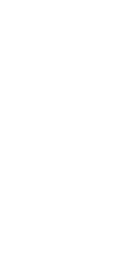
\includegraphics[width=0.3\textwidth]{WilliamsTube_PDARom.png}%
  }
  \par\vspace{0.3em}
  {\footnotesize\ttfamily The 256-glyph Character ROM atlas (16$\times$16 grid).}
\end{figure}

\begin{center}
{\small
\begin{tabular}{ccl}
  \toprule
  \textbf{Index Range} & \textbf{Count} & \textbf{Contents} \\
  \midrule
  0--31 & 32 & Box-drawing, block elements, symbols \\
  32--127 & 96 & Standard printable ASCII characters \\
  128--159 & 32 & Custom PDA icons \\
  160--255 & 96 & Inverted ASCII (mirrors 32--127) \\
  \bottomrule
\end{tabular}
}
\end{center}

% ============================================================================
% FREQUENTLY ASKED QUESTIONS
% ============================================================================
\newpage
\section{FREQUENTLY ASKED QUESTIONS}
\label{sec:faq}

\subsection{How does the display actually work?}

None of the logical operation of the device actually happens in an animation controller. The animation controller is used to respond to OSC commands that move the write head around, scale it, and toggle between drawing modes and font glyphs to render.

The visual sense of the render texture is built up as the write head scans around in front of an orthographic camera with depth-only culling, rapidly changing between the characters in the graphics ROM. The persistent render texture accumulates these writes like phosphor traces on a real CRT.

\subsection{Is a bitmap mode possible?}

Yes! The \textbf{IMG} program (see Section~\ref{sec:img}) renders arbitrary images in a bitmap display mode. Its appearance is much like a dot matrix printer or fax machine --- images are drawn character-by-character, each one truly transmitted from your computer into VRChat. Place images in the \texttt{assets/images} directory and select them from the list.

\subsection{Can I make my own programs?}

Anyone who's capable of writing code --- or brow-beating an AI into doing it for you --- can extend Yip OS, run a custom version, make their own programs, and/or make pull requests of programs to upstream.

The author at Foxipso Business Machines greatly fought the urge to make this whole thing a virtual machine executing programs written in assembly for a fictional, period-appropriate microcontroller, which would've been even more fun. But this current, saner approach merely requires C++ and supports all modern libraries and language features.

% ============================================================================
% SAFETY AND PRIVACY
% ============================================================================
\section{SAFETY AND PRIVACY}
\label{sec:safety}

\begin{warnbox}[CAUTION]
Depending on what features you enable, this device will display and allow interaction with your real, actual, potentially personal information to other users in VRChat. Avatar names, appropriate or inappropriate toggles, friend list, etc.

Depending on your interaction settings, other users may also be able to interact with the device --- they could cycle through your friends in VRCX, for example, or go through your list of recent avatars and make you change, or toggle things on and off on your avatar!

To combat this, \textbf{VRCX and AVTR are disabled by default} and require you to manually enable them in the Yip OS desktop app on your desktop, with your actual mouse and keyboard. You take any and all responsibility for your appropriate and considered use of this general purpose computing device.
\end{warnbox}

% ============================================================================
% TECHNICAL SPECIFICATIONS
% ============================================================================
\newpage
\section{TECHNICAL SPECIFICATIONS}
\label{sec:technical}

\subsection{Display}

\begin{center}
{\small
\begin{tabular}{ll}
  \toprule
  \textbf{Property} & \textbf{Value} \\
  \midrule
  Render Texture & 512$\times$512 R8G8B8A8\_UNORM \\
  Macro Atlas & 4096$\times$4096 R Compressed BC4 UNorm \\
  Visible Screen Area & 512$\times$264 pixels \\
  Text Grid & 40 columns $\times$ 8 rows \\
  Glyph Size & $\sim$12.8$\times$33 pixels \\
  Color Mode & Monochrome (customizable tint) \\
  Character ROM & 256 glyphs (16$\times$16 atlas) \\
  Write Speed & $\sim$70ms per glyph \\
  \bottomrule
\end{tabular}
}
\end{center}

\subsection{Synced Parameters (VRChat Network)}

\begin{center}
{\small
\begin{tabular}{llll}
  \toprule
  \textbf{Parameter} & \textbf{Type} & \textbf{Bits} & \textbf{Purpose} \\
  \midrule
  WT\_CursorX & Float & 8 & Horizontal position \\
  WT\_CursorY & Float & 8 & Vertical position \\
  WT\_CharLo & Int & 8 & Glyph index (0--255) \\
  WT\_ScaleA & Bool & 1 & Mode bit A \\
  WT\_ScaleB & Bool & 1 & Mode bit B \\
  PDA Enable & Bool & 1 & Enable/disable PDA \& Williams Tube \\
  \midrule
  \textbf{Total} & & \textbf{27} & \\
  \bottomrule
\end{tabular}
}
\end{center}

\subsection{Write Modes}
\label{sec:writemodes}

\begin{center}
{\small
\begin{tabular}{cclll}
  \toprule
  \textbf{ScaleA} & \textbf{ScaleB} & \textbf{Mode} & \textbf{Scale} & \textbf{Atlas} \\
  \midrule
  false & false & TEXT & 1/40 $\times$ 1/8 & Text ROM \\
  true & false & MACRO & 1.0 $\times$ 1.0 & Macro atlas \\
  false & true & CLEAR & 1.0 $\times$ 1.0 & (transparent fill) \\
  true & true & VQ & 1/32 $\times$ 1/32 & VQ codebook atlas \\
  \bottomrule
\end{tabular}
}
\end{center}

\subsection{Timing Reference}

\begin{center}
{\small
\begin{tabular}{lll}
  \toprule
  \textbf{Operation} & \textbf{Duration} & \textbf{Notes} \\
  \midrule
  Character write & $\sim$70ms & WRITE\_DELAY \\
  Mode switch & $\sim$40ms & SETTLE\_DELAY \\
  Screen clear & $\sim$300ms & Transparent fill \\
  Macro stamp & $\sim$110ms & Settle + write \\
  Full screen (brute) & $\sim$22s & 320 chars (avoid) \\
  Screen transition & $\sim$2--4s & Macro + dynamic \\
  Toggle response & $\sim$220ms & 2 char rewrites \\
  \bottomrule
\end{tabular}
}
\end{center}

\newpage
\subsection{Write Head Timing}

The following timing diagram illustrates the sequence of synced parameter states during a typical screen transition. The write head cycles through four modes: a transparent \textbf{CLEAR} to blank the screen, a full-screen \textbf{MACRO} stamp for the background, individual \textbf{TEXT} character writes for dynamic content, and \textbf{VQ} tile writes for bitmap graphics. Mode-change settle delays ($t_{settle}$) are required between each phase to allow the animation controller to process the new ScaleA/ScaleB state.

% write_head_timing.tex — Williams Tube Write Head Timing Diagram
% Shows parameter states during a typical screen transition:
%   CLEAR → MACRO stamp → TEXT writes → VQ bitmap writes

\newcommand{\wttbus}[5]{%
  % Bus value segment: #1=x1, #2=x2, #3=y-center, #4=label, #5=fill
  \fill[#5] ({#1+0.12},{#3+0.2}) -- ({#2-0.12},{#3+0.2}) -- ({#2},{#3})
    -- ({#2-0.12},{#3-0.2}) -- ({#1+0.12},{#3-0.2}) -- ({#1},{#3}) -- cycle;
  \draw ({#1},{#3}) -- ({#1+0.12},{#3+0.2}) -- ({#2-0.12},{#3+0.2})
    -- ({#2},{#3}) -- ({#2-0.12},{#3-0.2}) -- ({#1+0.12},{#3-0.2}) -- cycle;
  \node[font=\tiny\ttfamily] at ({(#1+#2)/2},{#3}) {#4};%
}
\newcommand{\wttstl}[3]{%
  % Settle/unknown segment: #1=x1, #2=x2, #3=y-center
  \fill[gray!10] ({#1},{#3-0.2}) rectangle ({#2},{#3+0.2});
  \draw ({#1},{#3+0.2}) -- ({#2},{#3+0.2});
  \draw ({#1},{#3-0.2}) -- ({#2},{#3-0.2});
  \draw[gray!40] ({#1},{#3+0.2}) -- ({#2},{#3-0.2});
  \draw[gray!40] ({#1},{#3-0.2}) -- ({#2},{#3+0.2});%
}

\begin{figure}[H]
\centering
\resizebox{0.95\textwidth}{!}{%
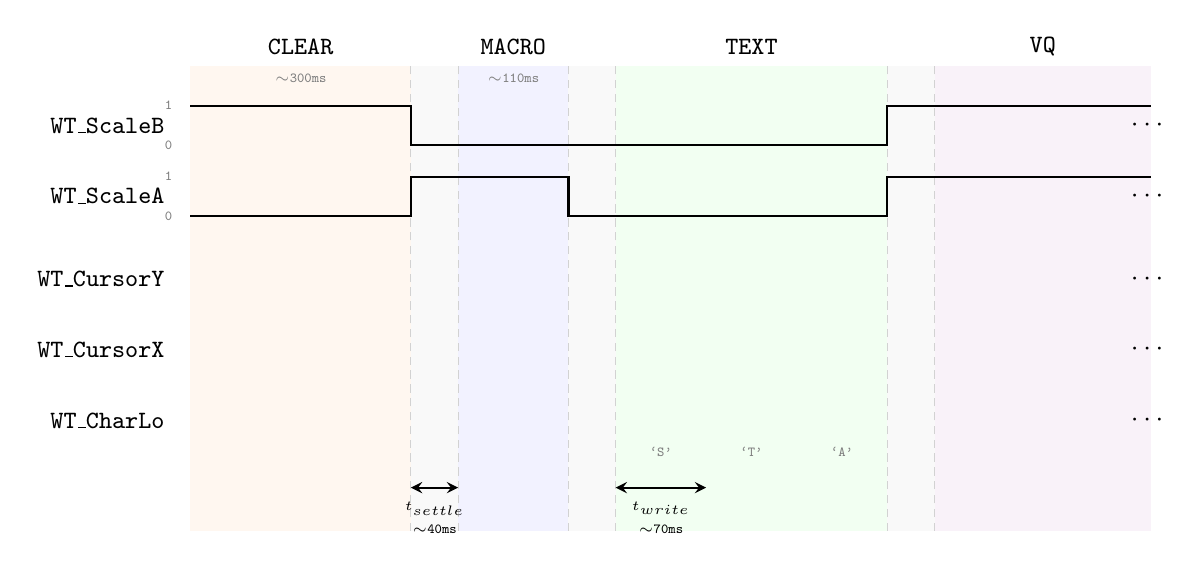
\begin{tikzpicture}[y=1cm, >=stealth]

% ================================================================
% Time positions (in cm):
%   CLEAR:   0.0 -- 2.8
%   Settle:  2.8 -- 3.4
%   MACRO:   3.4 -- 4.8
%   Settle:  4.8 -- 5.4
%   TEXT:    5.4 -- 8.85  (3 chars: 5.4--6.55, 6.55--7.7, 7.7--8.85)
%   Settle:  8.85 -- 9.45
%   VQ:      9.45 -- 11.85 (2 tiles: 9.45--10.65, 10.65--11.85)
%   Dots:    ~12.1
% ================================================================

% ================================================================
% Phase background shading
% ================================================================
\fill[orange!6]  (0, -0.5) rectangle (2.8, 5.4);
\fill[gray!5]    (2.8, -0.5) rectangle (3.4, 5.4);
\fill[blue!5]    (3.4, -0.5) rectangle (4.8, 5.4);
\fill[gray!5]    (4.8, -0.5) rectangle (5.4, 5.4);
\fill[green!5]   (5.4, -0.5) rectangle (8.85, 5.4);
\fill[gray!5]    (8.85, -0.5) rectangle (9.45, 5.4);
\fill[violet!5]  (9.45, -0.5) rectangle (12.2, 5.4);

% ================================================================
% Phase separator lines
% ================================================================
\foreach \tx in {2.8, 3.4, 4.8, 5.4, 8.85, 9.45} {
  \draw[densely dashed, gray!35] (\tx, -0.5) -- (\tx, 5.4);
}

% ================================================================
% Phase labels (top)
% ================================================================
\node[font=\small\ttfamily\bfseries] at (1.4, 5.65) {CLEAR};
\node[font=\small\ttfamily\bfseries] at (4.1, 5.65) {MACRO};
\node[font=\small\ttfamily\bfseries] at (7.125, 5.65) {TEXT};
\node[font=\small\ttfamily\bfseries] at (10.825, 5.65) {VQ};
\node[font=\tiny\ttfamily, gray] at (1.4, 5.25) {$\sim$300ms};
\node[font=\tiny\ttfamily, gray] at (4.1, 5.25) {$\sim$110ms};

% ================================================================
% Signal: WT_ScaleB — low=4.4, high=4.9
% CLEAR(H) → MACRO(L) → TEXT(L) → VQ(H)
% ================================================================
\node[font=\small\ttfamily, anchor=east] at (-0.2, 4.65) {WT\_ScaleB};
\draw[thick] (0, 4.9) -- (2.8, 4.9)
  -- (2.8, 4.4) -- (8.85, 4.4)
  -- (8.85, 4.9) -- (12.2, 4.9);
% LOW reference
\draw[dotted, gray!25] (2.8, 4.4) -- (2.8, 4.4);

% ================================================================
% Signal: WT_ScaleA — low=3.5, high=4.0
% CLEAR(L) → MACRO(H) → TEXT(L) → VQ(H)
% ================================================================
\node[font=\small\ttfamily, anchor=east] at (-0.2, 3.75) {WT\_ScaleA};
\draw[thick] (0, 3.5) -- (2.8, 3.5)
  -- (2.8, 4.0) -- (4.8, 4.0)
  -- (4.8, 3.5) -- (8.85, 3.5)
  -- (8.85, 4.0) -- (12.2, 4.0);

% HIGH / LOW annotations
\node[font=\tiny\ttfamily, gray, anchor=east] at (-0.1, 4.9) {1};
\node[font=\tiny\ttfamily, gray, anchor=east] at (-0.1, 4.4) {0};
\node[font=\tiny\ttfamily, gray, anchor=east] at (-0.1, 4.0) {1};
\node[font=\tiny\ttfamily, gray, anchor=east] at (-0.1, 3.5) {0};

% ================================================================
% Signal: WT_CursorY — bus, center=2.7
% CLEAR/MACRO: 0x80 (centered), TEXT/VQ: 0x00 (row/tile 0)
% ================================================================
\node[font=\small\ttfamily, anchor=east] at (-0.2, 2.7) {WT\_CursorY};
\wttbus{0}{2.8}{2.7}{0x80}{orange!12}
\wttstl{2.8}{3.4}{2.7}
\wttbus{3.4}{4.8}{2.7}{0x80}{blue!10}
\wttstl{4.8}{5.4}{2.7}
\wttbus{5.4}{8.85}{2.7}{0x00}{green!10}
\wttstl{8.85}{9.45}{2.7}
\wttbus{9.45}{11.85}{2.7}{0x00}{violet!10}

% ================================================================
% Signal: WT_CursorX — bus, center=1.8
% CLEAR/MACRO: 0x80, TEXT: steps through columns, VQ: steps through tiles
% ================================================================
\node[font=\small\ttfamily, anchor=east] at (-0.2, 1.8) {WT\_CursorX};
\wttbus{0}{2.8}{1.8}{0x80}{orange!12}
\wttstl{2.8}{3.4}{1.8}
\wttbus{3.4}{4.8}{1.8}{0x80}{blue!10}
\wttstl{4.8}{5.4}{1.8}
\wttbus{5.4}{6.55}{1.8}{0x01}{green!10}
\wttbus{6.55}{7.7}{1.8}{0x02}{green!10}
\wttbus{7.7}{8.85}{1.8}{0x03}{green!10}
\wttstl{8.85}{9.45}{1.8}
\wttbus{9.45}{10.65}{1.8}{0x00}{violet!10}
\wttbus{10.65}{11.85}{1.8}{0x01}{violet!10}

% ================================================================
% Signal: WT_CharLo — bus, center=0.9
% CLEAR: 0x00, MACRO: glyph index, TEXT: ASCII, VQ: codebook index
% ================================================================
\node[font=\small\ttfamily, anchor=east] at (-0.2, 0.9) {WT\_CharLo};
\wttbus{0}{2.8}{0.9}{0x00}{orange!12}
\wttstl{2.8}{3.4}{0.9}
\wttbus{3.4}{4.8}{0.9}{0x03}{blue!10}
\wttstl{4.8}{5.4}{0.9}
\wttbus{5.4}{6.55}{0.9}{0x53}{green!10}
\wttbus{6.55}{7.7}{0.9}{0x54}{green!10}
\wttbus{7.7}{8.85}{0.9}{0x41}{green!10}
\wttstl{8.85}{9.45}{0.9}
\wttbus{9.45}{10.65}{0.9}{0x1A}{violet!10}
\wttbus{10.65}{11.85}{0.9}{0x7F}{violet!10}

% ASCII character annotations below CharLo during TEXT phase
\node[font=\tiny, gray] at ({(5.4+6.55)/2}, 0.5) {\texttt{`S'}};
\node[font=\tiny, gray] at ({(6.55+7.7)/2}, 0.5) {\texttt{`T'}};
\node[font=\tiny, gray] at ({(7.7+8.85)/2}, 0.5) {\texttt{`A'}};

% ================================================================
% Continuation dots
% ================================================================
\foreach \yy in {4.65, 3.75, 2.7, 1.8, 0.9} {
  \node[font=\normalsize] at (12.15, \yy) {$\cdots$};
}

% ================================================================
% Timing annotations
% ================================================================
% Settle delay
\draw[<->, thick] (2.8, 0.05) -- (3.4, 0.05);
\node[font=\tiny\ttfamily, below] at (3.1, 0.0) {$t_{settle}$};
\node[font=\tiny\ttfamily, below] at (3.1, -0.3) {$\sim$40ms};

% Write delay (one character)
\draw[<->, thick] (5.4, 0.05) -- (6.55, 0.05);
\node[font=\tiny\ttfamily, below] at (5.975, 0.0) {$t_{write}$};
\node[font=\tiny\ttfamily, below] at (5.975, -0.3) {$\sim$70ms};

\end{tikzpicture}%
}

\par\vspace{0.3em}
{\footnotesize\ttfamily Figure 3: Write head parameter timing during a typical screen transition.
WT\_ScaleA and WT\_ScaleB select the write mode (see Section~\ref{sec:writemodes}).
WT\_CursorX/Y position the write head. WT\_CharLo selects the glyph, macro index,
or VQ codebook entry. Hatched regions indicate settle delays between mode changes.
TEXT values shown: 0x53=`S', 0x54=`T', 0x41=`A'.}
\end{figure}


% ============================================================================
% COMPANION SOFTWARE
% ============================================================================
\newpage
\section{COMPANION SOFTWARE}
\label{sec:companion}

The Desktop Companion is a C++ application that runs on your PC and drives the Yip-Boi's display over OSC. It must be running whenever you want the PDA to function. The companion application runs on both \textbf{Windows} and \textbf{Linux}.

\subsection{Installation}

Insert the Desktop Companion Software disk (3.5'' floppy) into your PC's disk drive. If your PC does not have a 3.5'' drive, the software is also available for download from your Foxipso dealer's BBS. Or from the new invention of the World Wide Web, at \url{https://github.com/InconsolableCellist/YipOS}.

\subsubsection*{Linux}

The companion application builds and runs natively on Linux. Audio capture (for the CC program) uses PulseAudio, which is also supported by PipeWire's compatibility layer. Vulkan is used for GPU-accelerated Whisper inference. Install the following development packages before building:

\begin{itemize}[leftmargin=2em, nosep]
  \item OpenGL, libcurl, PulseAudio, and Vulkan development headers
  \item \texttt{glslc} (Vulkan shader compiler)
\end{itemize}

\noindent See the project README for distribution-specific package names.

% ============================================================================
% TROUBLESHOOTING
% ============================================================================
\section{TROUBLESHOOTING}
\label{sec:troubleshooting}

\subsection{The display is blank in VRChat!}
\label{sec:blankdisplay}

There are several common causes for a blank display in VRChat:

\begin{itemize}[leftmargin=2em, nosep]
  \item \textbf{Unity is stealing the OSC ports.} If Unity is open with the Williams Tube OSC Sender/Receiver scripts listening on the default ports, Yip OS can't connect. Close Unity, toggle OSC on and off on your avatar in VRChat, reopen Yip OS, and try again. You should see an OSC Query notification in VRChat when Yip OS launches.
  \item Press \key{BACK} on the PDA to redraw the Home screen.
  \item Disable and re-enable OSC in your VRChat radial menu (Action Menu $\rightarrow$ Options $\rightarrow$ OSC).
  \item Reset your avatar's OSC config in your radial menu.
  \item Change out of your avatar and back into it.
  \item Toggle the PDA off and on in your radial menu, then press \key{BACK} in Yip OS.
  \item Verify the avatar prefab is correctly installed (see Section~\ref{sec:setup}).
\end{itemize}

\subsection{The spinner isn't spinning}

The companion software is not running or has lost connection. Restart the companion app and verify OSC is enabled in VRChat.

\subsection{Characters appear garbled}

Write delay may be too fast. Try setting write speed to \textbf{SLOW} in CONF (see Section~\ref{sec:conf}), or adjust the write delay slider in the \textbf{Display} tab of the desktop app.

\subsection{The screen flashes every so often}

The auto-refresh feature is enabled. This periodically redraws the entire screen to correct any display corruption, but causes a visible flash. Set \textbf{REFR} to \textbf{OFF} in the CONF program for best performance (see Section~\ref{sec:conf}).

\subsection{Touch inputs don't register}

If nothing is displaying at all, see Section~\ref{sec:blankdisplay} above. If you can see graphics on the display, check the bottom-left of the status bar for a lock icon. If visible, the device is locked --- tap \key{SEL} three times to exit lock mode (see Section~\ref{sec:lock}).

\subsection{Remote users see missing characters}

Your write speed is too fast for network sync. Switch to SLOW in CONF for reliable remote viewing. Some programs, like IMG, will do one pass quickly and then slow down to sync data for remote players.

\subsection{My inputs aren't registering!}

\textbf{ALOCK} (autolock) is enabled by default. Check the bottom-left of the status bar --- if you see the lock icon, press \key{SEL} three times rapidly to unlock. You can adjust the autolock timeout or disable it entirely in the CONF program (see Section~\ref{sec:conf}).

\subsection{My output looks misaligned on the CRT!}

\begin{itemize}[leftmargin=2em, nosep]
  \item Check the \textbf{Display} tab in the Yip OS desktop app and reset \textbf{Y Offset}, \textbf{Y Scale}, and \textbf{Y Curve}.
  \item Check your Williams Tube asset in the Hierarchy and make sure you don't have any overrides affecting its positioning or scale.
  \item Delete the asset from your avatar and Project View and import fresh.
\end{itemize}

\subsection{When people move around I see weird lines or nametags in the CRT}

The Williams Tube camera lives on the \textbf{UiMenu} layer, out of necessity, and anything else that draws to that layer (such as nametags) will be added to the Render Texture. Refresh the screen (such as pressing \key{BACK}) to clear it.

% ============================================================================
% APPENDICES
% ============================================================================
\newpage
\appendix

\section{QUICK REFERENCE CARD}
\label{sec:quickref}

\begin{screenbox}[title={\color{crtgreen}CONTROLS SUMMARY}]
\begin{verbatim}
 BUTTONS:                     DISPLAY:
   [BACK]  Back / Home          Inverted text = touchable
   [PGUP]  Page Up              Spinner = connection OK
   [PGDN]  Page Down            Lock icon = locked
   [SEL]   Select/Context       * = notification waiting
   [JOY]   Scroll Down          Clock = 24h local time
 TOUCHSCREEN:
   5 x 3 grid (15 zones)     NAVIGATION:
   Index finger required        Home -> tap tile -> program
                                [BACK] returns one screen
 LIST SELECTION:
   [JOY] cycles items
   [SEL] selects item
\end{verbatim}
\end{screenbox}

\section{GLOSSARY}
\label{sec:glossary}

\begin{description}[style=nextline, leftmargin=1em, font=\ttfamily\bfseries]
  \item[Character ROM]
    The 256-glyph font atlas supplied on 3.5'' floppy. Defines every displayable character and icon.

  \item[CRT]
    Cathode Ray Tube. The display technology being lovingly emulated.

  \item[Glyph]
    A single character or symbol from the Character ROM.

  \item[Inverted Video]
    Foreground and background colors swapped. Indicates a touchable element.

  \item[Macro Glyph]
    A pre-rendered full-screen image stamped in one write cycle. The secret to fast screen transitions.

  \item[NVRAM]
    Non-volatile RAM. Stores configuration and selections between power cycles. Clearable via CONF.

  \item[OSC]
    Open Sound Control. UDP protocol linking the companion software to VRChat.

  \item[OSC Query]
    Service discovery protocol using mDNS/DNS-SD and HTTP. Lets VRChat and OSC apps find each other automatically without manual port configuration.

  \item[Render Texture]
    The persistent 512$\times$512 framebuffer. Glyphs accumulate like phosphor traces.

  \item[Spinnyboi]
    The rotating status cursor. Technical term. See Section~\ref{sec:spinner}.

  \item[Williams Tube]
    The rendering pipeline. Named after the Williams-Kilburn tube (1947), one of the first electronic memory devices.

  \item[Write Head]
    The shader quad that deposits individual glyphs onto the render texture.
\end{description}

\section{SUPPORT}
\label{sec:support}

Feel free to reach out to Foxipso using any of the following methods for support or updates:

\begin{description}[style=nextline, leftmargin=1em, font=\bfseries\ttfamily, nosep]
  \item[Linktr.ee] \url{https://foxipso.com}
  \item[Gumroad] \url{https://foxipso.gumroad.com/}
  \item[Jinxxy] \url{https://jinxxy.com/foxipso}
  \item[X/Twitter] \url{https://twitter.com/TheFoxipso}
  \item[Discord] foxipso
  \item[Foxipso's Den Discord] \url{https://discord.gg/2jYw4swm3X}
\end{description}

\section{WARRANTY}
\label{sec:warranty}

Foxipso Business Machines warrants the Yip-Boi PDA (Model YB-1) against defects in materials and workmanship for a period of ninety (90) virtual days from the date of original purchase. This warranty does not cover:

\begin{itemize}[leftmargin=2em, nosep]
  \item Damage caused by improper installation of the Character ROM disk
  \item Phosphor burn-in resulting from displaying the same screen for extended periods (this is not actually possible, but we're covering our bases)
  \item Damage caused by exposure to water, fire, or the VRChat particle limit
  \item Embarrassment resulting from other players reading your system stats
  \item Other players changing your avatar via the AVTR program
  \item Distressing content received via the CHAT program from other Yip-Boi owners
\end{itemize}

To obtain warranty service, contact your authorized Foxipso dealer with proof of purchase and a detailed description of the defect. Do \textit{not} attempt to service the unit yourself. There are no user-serviceable parts inside. We checked.

\vfill
\begin{center}
\textcolor{rulecolor}{\rule{0.5\textwidth}{0.8pt}}\\[0.5em]
{\footnotesize\ttfamily
Me here at Foxipso Business Machines hopes that you'll enjoy\\
using your new Yip-Boi arm-worn computer!\\[0.5em]
FOXIPSO BUSINESS MACHINES, INC.\\[0.3em]
Part No. FBM-YB-001-EN Rev.1.0.3 --- 2026}
\end{center}

\end{document}
